



\section{System design}

    This section describes the overall design of the simulation system
    and the ways in which it can be used, as well as some notes
    regarding its implementation.


\subsection{Overview}

\begin{figure}[htb]
        \centering
        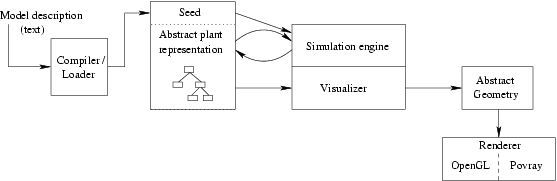
\includegraphics[width=12cm,angle=0]{images/system_overview}
        \label{fig:sys1}
    \caption{Overview of the system}
\end{figure}


    The major part of the application consists of two modules, the
    simulation engine and the visualization module. The simulation
    works on an abstract representation of the plant structure which
    contains necessary information to both control the simulation and
    to enable the visualization module to generate an geometric
    representation of the simulated plant. 

    The abstract geometric output from the visualization module can
    then be used as input to a renderer backend, we have implemented
    two such systems, one for real-time visualizations using OpenGL
    and one for batch generation of high-quality images using Povray.

    The level of the abstract geometric representation is chosen high
    enough to allow for a number of different rendering techniques
    while still making it possible to describe the structure in
    sufficient detail.


\subsubsection{Model}

    In the modeling stage a seed is constructed using one of the
    supported embedded languages.


\subsubsection{Loading}


    The textual representation is transformed into internal
    representation by a compiler and a loader. By using the same language
    in both model descriptions and the implementation of the
    system we get this functionality for free.


\subsubsection{Simulation}

   The simulation engine initializes the internal representation from
   the seed constructed from the model, and iteratively modifies this
   representation according to inputs given by the user representing
   the environment of the simulation.


\subsubsection{Visualization}

    When an visualization is demanded, the internal representation is
    traversed and an abstract geometric representation is constructed. 
    Currently a number of primitives for building
    branches and leaves are available, but this set can easily be
    extended if support for more advanced structures is required, such
    as flowers and various forms of fruits.

\label{system:geomrep}


\subsubsection{Renderer}

    The renderer provides a visual representation of the abstract
    geometry by translating it into either OpenGL commands or a format
    understood by a raytracing system, such as Povray. Many different
    rendering technologies may be used here, the two provided can be
    seen as examples of the possibilities.


\subsection{Implementation}

    The system can be used in two ways, either as a standalone
    application used to develop models in an interactive way, or as an
    embedded library in another applications (a game, for example).
    The standalone applications provides a simple graphical interface
    where the user can develop programs and watch the resulting plants
    interactively. 

    There are two interfaces available for embedding, either the
    abstract geometry is used and parsed by the host, or our
    OpenGL-renderer is used directly. The former approach is
    recommended for serious use since it gives full power to the host
    regarding presentation and rendering decisions.


\subsubsection{Tools}
 
    The simulation modules and development environment is implemented
    using Haskell and ghc together with a number of libraries. A
    number of extension to pure Haskell98 are used, either for
    performance reasons (the ST-monad in one of the approaches) or
    programmatic convenience and abstraction purposes
    (multi.param.type classes, implicit parameters and existential
    types).

    The GUI is written with gtk+hs using HOpenGL for visualization of models. 

    Povray\cite{povray} is used for raytraced renderings.

\subsubsection{Language choice}

    Haskell was chosen for a number of reasons, mainly because we
    know it well and thought it was very suitable for our purpose
    (quick prototyping, ease of abstraction, embedding domain specific
    language, ...)


\subsubsection{DSELS}

    Much have already been said about advantages and disadvantages
    of embedding a domain specific language in an already existing host
    language, we have largely arrived at the same position
    with a few additions, one advantage not mentioned very often, at least
    not explicitly, is the ease of which functionality can be moved back
    and forth between the host implementation and the embedded part.
    This is of great help especially when the problem is a bit fuzzy, when
    we do not know exactly which functionally is needed in the embedded
    language. A pure domain solution which is found to be generally
    useful, or in need of optimization only possible in the core, can be
    directly considered to be part of the language, since the host and
    the embedded parts are the same.




